\section{Overview of neutron \el\ experiments}
In neutron elastic scattering measurements, the same time-of-flight techniques are used:
given a "starting gun" when neutrons are produced and the neutron arrival time
at a time-of-flight detector, the neutron energy can be calculated.
However, in contrast to total cross section measurements, neutron elastic scattering
measurements require a monoenergetic neutron beam so that elastically-scattered
neutrons can be isolated. Unlike transmission measurements (e.g., total cross
sections), which measure the neutron \el\ and \rxn\ scattering cross sections integrated
over all solid angles, neutron \el\ cross sections are measured differentially with respect to 
solid angle. To measure the angular dependence, one or more time-of-flight detectors
are moved around the scattering sample on a large goniometer. As the differential cross section 
drops precipitously at large scattering angles, more beam time must be spent at
large angles to generate sufficient statistics.

In transmission measurements, the time-of-flight detector is typically placed
very far from the scattering sample so that it subtends an extremely small solid
angle so that only unattenuated particles are detected.
For example, in the neutron \tot\ experimental setup described in Chapter
\ref{TCSExperiment}, the scintillator of the time-of-flight detector subtended
4.5x10$^{-6}$ steradians from the point of view of the samples. Thus, the
contribution to background from isotropic $\gamma$-ray production in the samples is negligible.
In differential measurements,
background from $\gamma$-ray production in the samples may exceed the signal
from elastically-scattered neutrons, especially at backward angles where the elastic
cross section is lowest. Pulse-shape discrimination (PSD) techniques must be used to filter out 
$\gamma$ rays, leaving only events from elastically-scattered neutrons.

\subsection{Pulse-Shape Discrimination (PSD)}
To identify neutron- and gamma-induced detector events, pulse-shape discrimination
relies on the different energy deposition modes of neutrons and $\gamma$ rays.
A liquid scintillator must be selected that
possesses excited states capable of both prompt fluorescence (from a singlet
state) and delayed phosphorescence (from a triplet state) accessible through
intersystem crossing, as shown in Figure \ref{JablonskiExample}. During an experiment, incident 
neutrons deposit energy by collision with scintillator nuclei.
These recoiling nuclei decelerate rapidly in the scintillating
medium via Coulombic interactions. In contrast, incident $\gamma$ rays interact primarily with
atomic electrons, which have smaller linear energy transfer rates during their
recoil. For the same total energy deposition, neutron-initiated events produce a higher 
concentration of excited states than $\gamma$-ray-initiated events. The increased
concentration of excited states facilitates intersystem crossing, producing
a small population of triplet-state molecules with far-higher lifetimes.
By analyzing the tail of the light output signal after the prompt decay of
singlet states, neutrons and $\gamma$-rays can be distinguished.
Recently, machine learning techniques have been
applied to PSD data of this type to further improve discrimination \cite{Doucet2018}.

\begin{figure}[h]
    \centering
    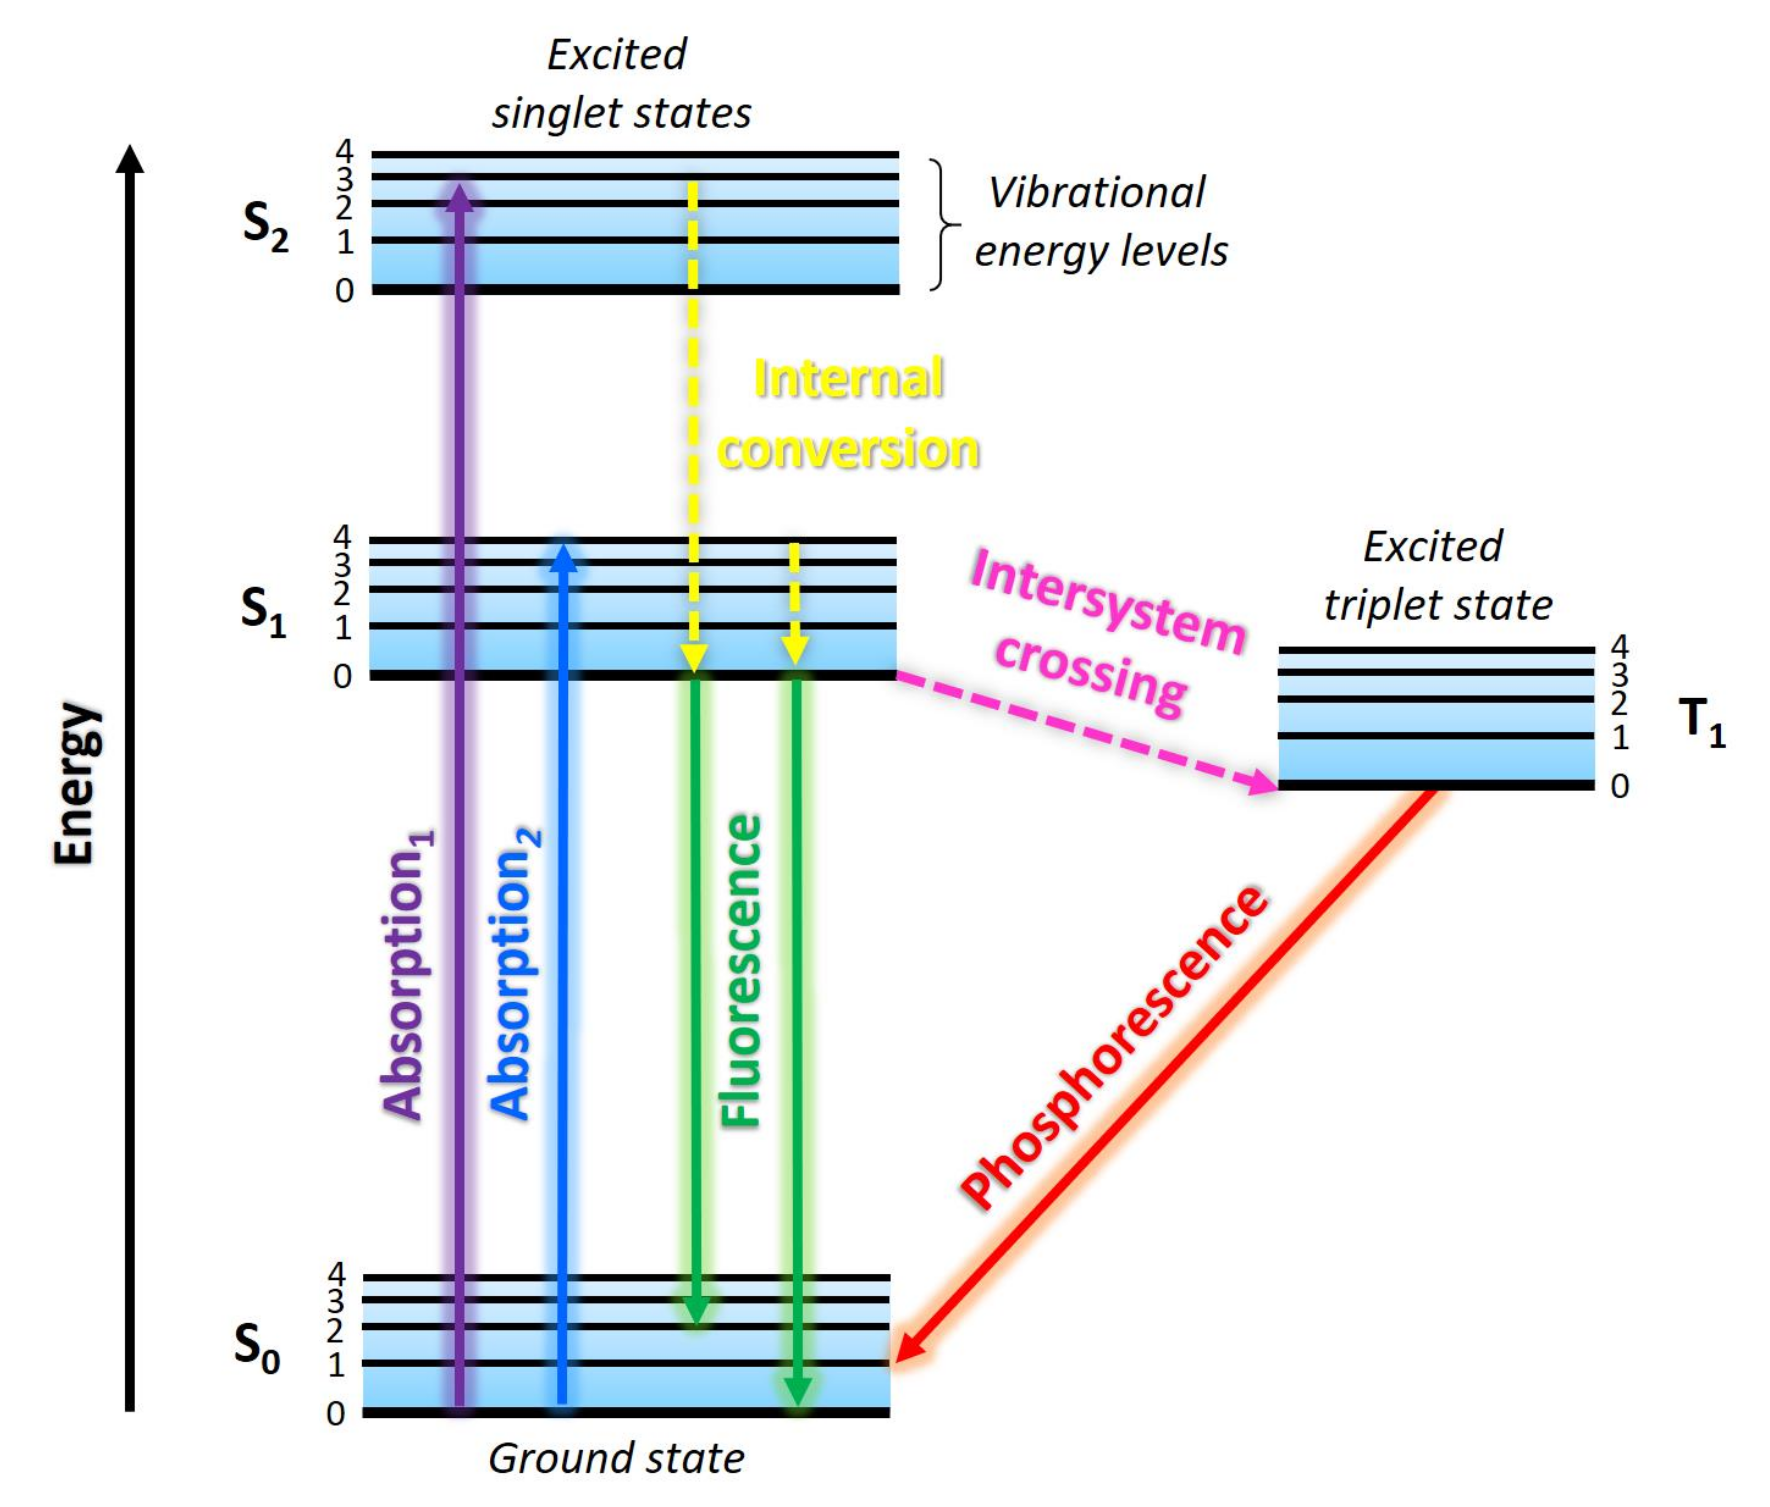
\includegraphics[width = 0.9\textwidth]{figures/JablonskiExample_KangDissertation.png}
    \caption[Example Jablonski diagram for organic scintillator]
    {
        Example Jablonski diagram for an organic scintillator used for
        pulse-shape discrimination. After initial excitation to a higher
        electronic manifold, energy is shed non-radiatively by internal
        conversion on the picosecond timescale. If the first vibrational state of the S1
        manifold is reached, rapid decay to the S0 manifold occurs on the
        nanosecond timescale. Alternatively, the system may undergo intersystem
        crossing to the T1 manifold, where it reaches the lowest vibrational
        state. The T1-S0 transition is quantum-mechanically-forbidden,
        dramatically increasing the lifetime of the T1 state and leading to
        delayed light output, or phosphorescence. Figure used with permission 
        from J. Kang \cite{KangPhDThesis}. 
    }
    \label{JablonskiExample}
\end{figure}

In our \snTwelveFour\ neutron \el\ cross section measurements presented below,
we used both PSD data of this kind and the pulse height of each
event to segregate neutrons from $\gamma$-rays (see Figure \ref{PHPSDPlot} in Chapter
\ref{ECSAnalysis}). Our approach follows similar neutron \el\ measurements
conducted at TUNL over the last three decades,
including measurements on $^{116,120}$Sn conducted by Guss et al.
\cite{Guss1989, GussPhDThesis} to which we later compare our results.

\section{Sample Preparation}
The same \snTwelveNatFour\ samples used in the neutron \tot\ experiment (see Chapter
\ref{TCSExperiment}) were used for our neutron
\el\ measurements without modification. Two additional samples, one of graphite and one
polyethylene, were provided by the TUNL facility so that our measurements could
be normalized using the extremely-well-known (n,p) elastic cross section. The
details of this normalization are given in Chapter \ref{ECSAnalysis}.
The physical characteristics of all the samples are given in 
\ref{ECSSampleTable}.

\begin{table}[ht]
    \caption[Physical characteristics of samples used for neutron \el\
    measurements]
    {
        Physical characteristics of samples used for the neutron \el\
        measurements. For isotopically-enriched samples, the natural abundance
        of the enriched isotope and the isotopic fraction of the sample are
        given.
    }
    \label{ECSSampleTable}
    \begin{center}
        \begin{tabular}{ c c c c c c c }
            \hline
            Isotope & Length & Diameter
            & Mass & Nat. Abund. & Sample Purity\\
                 & [mm] & [mm] & [g] & [\%] & [\%]\\
            \hline

            $^{\text{nat}}$C & 23.58 & 9.39 & 2.924 & - & -\\
            (CH$_{2}$)$_{n}$ & 22.70 & 14.18 & 3.389 & - & -\\

            $^{112}$Sn & 13.65(3) & 8.245(5) &
            4.9720 & 0.97 & 99.9\\
            $^{\text{nat}}$Sn & 13.68(3) & 8.245(5) &
            5.3263 & - & -\\
            $^{124}$Sn & 13.73(3) & 8.245(5) &
            5.5492 & 5.79 & 99.9\\

            \hline
        \end{tabular}
    \end{center}
\end{table}

\section{Experimental Facility at TUNL}
We conducted our neutron \el\ measurements at the neutron TOF
beamline of the Triangle Universities Nuclear Laboratory (TUNL) facility
(diagrammed in Fig. \ref{ExperimentalSetupTUNL}) in 2017 and 2018.
Incident deuterons, supplied by the
facility's variable-energy tandem Van De Graaf accelerator, impinged on a deuterium
gas cell to produce a forward-focused neutron beam via the d(d,n)$^{3}$He reaction.
Two measurements, one for 11 MeV neutrons and one for 17 MeV neutrons, were
conducted. For the 11 MeV measurement, the neutron beam energy distribution
had FWHM of [insert beam energy distribution FWHM] MeV. For the 17 MeV
measurement, the FWHM was [insert beam energy FWHM]. The deuterium gas cell
was backed with a fresh tantalum beam stop to prevent unreacted deuterons from
reaching the samples. 

The production samples (\snTwelve, \snFour, and a blank) were suspended several
cm downstream of the gas well in a vertically-aligned wire basket apparatus.
In addition to the production runs, a few normalization runs were taken
with the TUNL-supplied samples (graphite, polyethylene, and a blank).
Between runs, samples were rotated into position
with a hand-actuated pulley. Sample alignment with the gas cell was confirmed
by telescopic sight. Neutrons scattering off the samples were recorded by one
of the two main time-of-flight
detectors, designated ``4M" and ``6M", roughly 4 and 6 meters away from the target.
These detectors were mounted on large, movable carriages, or "arms",
that could be rotated to different angles independently so that two angular
measurements could be conducted simultaneously. By recessing the detectors deep within
the arms' heavy shielding, only neutrons entering the arm at a precise angle
were counted.

To further reduce room background and to screen direct neutrons the gas cell,
an ensemble of "shadow bars" (wedge-shaped tungsten bricks)
were used to adjust the aperture at the entrance to the arms. After an arm's
angle was changed, the shadow bars were aligned by hand so that the
detector within the arm had no line-of-sight to the gas cell or the
shielding of the other arm. Any configuration in which the arms were in opposition (i.e., the
angle between the arms was 180$\pm$20 degrees) could allow neutrons scattered
from one arm to enter the detector of the other arm, so these configurations were avoided.

Besides the time-of-flight detectors installed in the arms, a ceiling monitor
detector (CMON) and zero-degree detector aligned with the beam (ZDEG) were used
to record beam flux. In addition, a capacitive pickoff signal
from the accelerator was collected to serve as a time-of-flight
(TOF) stop signal any time an event was recorded on one of the four neutron
detectors. Prior to production, detectors were gain-matched and calibrated with $^{137}$Cs
and $^{22}$Na sources. For the 4M (6M) detector, a time resolution of [insert
resolution] ns was established.

\begin{figure}[h]
    \centering
    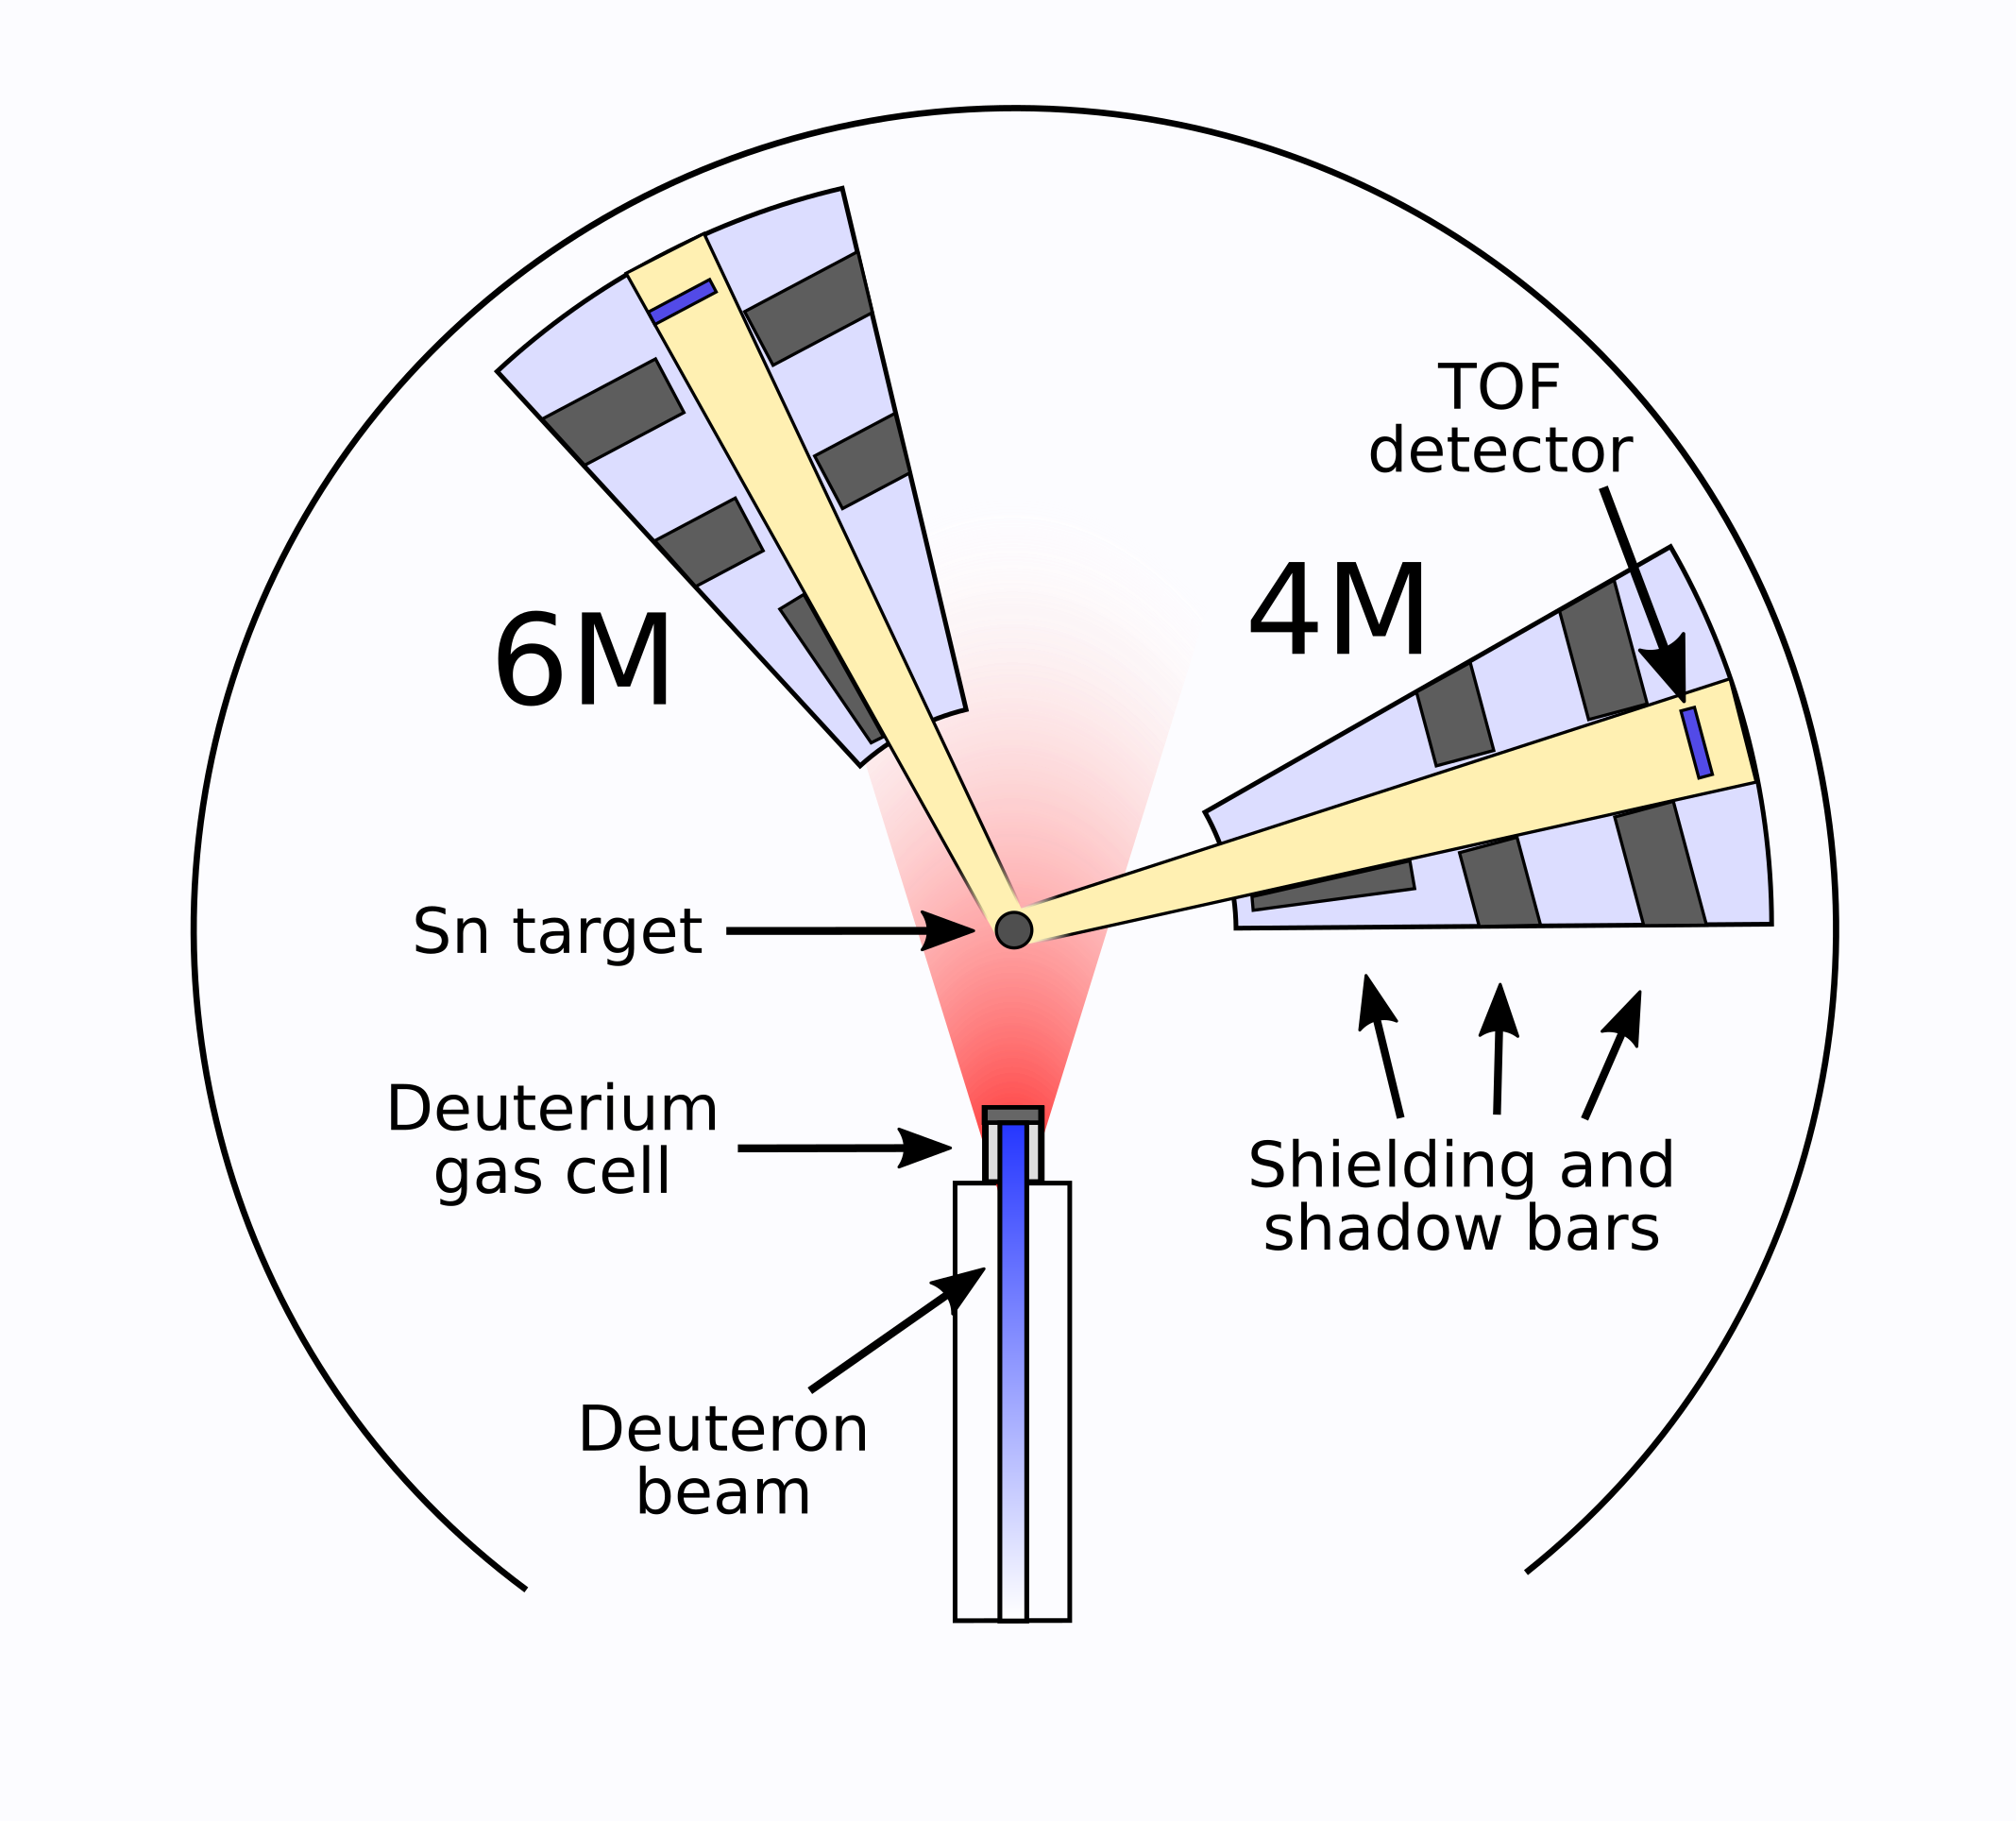
\includegraphics[width = 0.9\textwidth]{figures/ExperimentalSetupTUNL.png}
    \caption[Diagram of the neutron TOF room at TUNL] 
    {
        Diagram of the neutron TOF room at TUNL. Neutrons are produced by d(d,n)$^{3}$He reaction in
        a small gas cell, forming a forward-focused cone (in red). They scatter
        off the sample into one of the detector arms, labeled 4M and 6M, where the neutron
        times-of-flight are recorded. Another shielded detector (not pictured), suspended from the 
        ceiling, serves as a flux monitor so that absolute cross sections can be
        recovered. The angle of each detector arm is read from a goniometer in
        the center of the room.
    }
    \label{ExperimentalSetupTUNL}
\end{figure}

\begin{figure}[h]
    \centering
    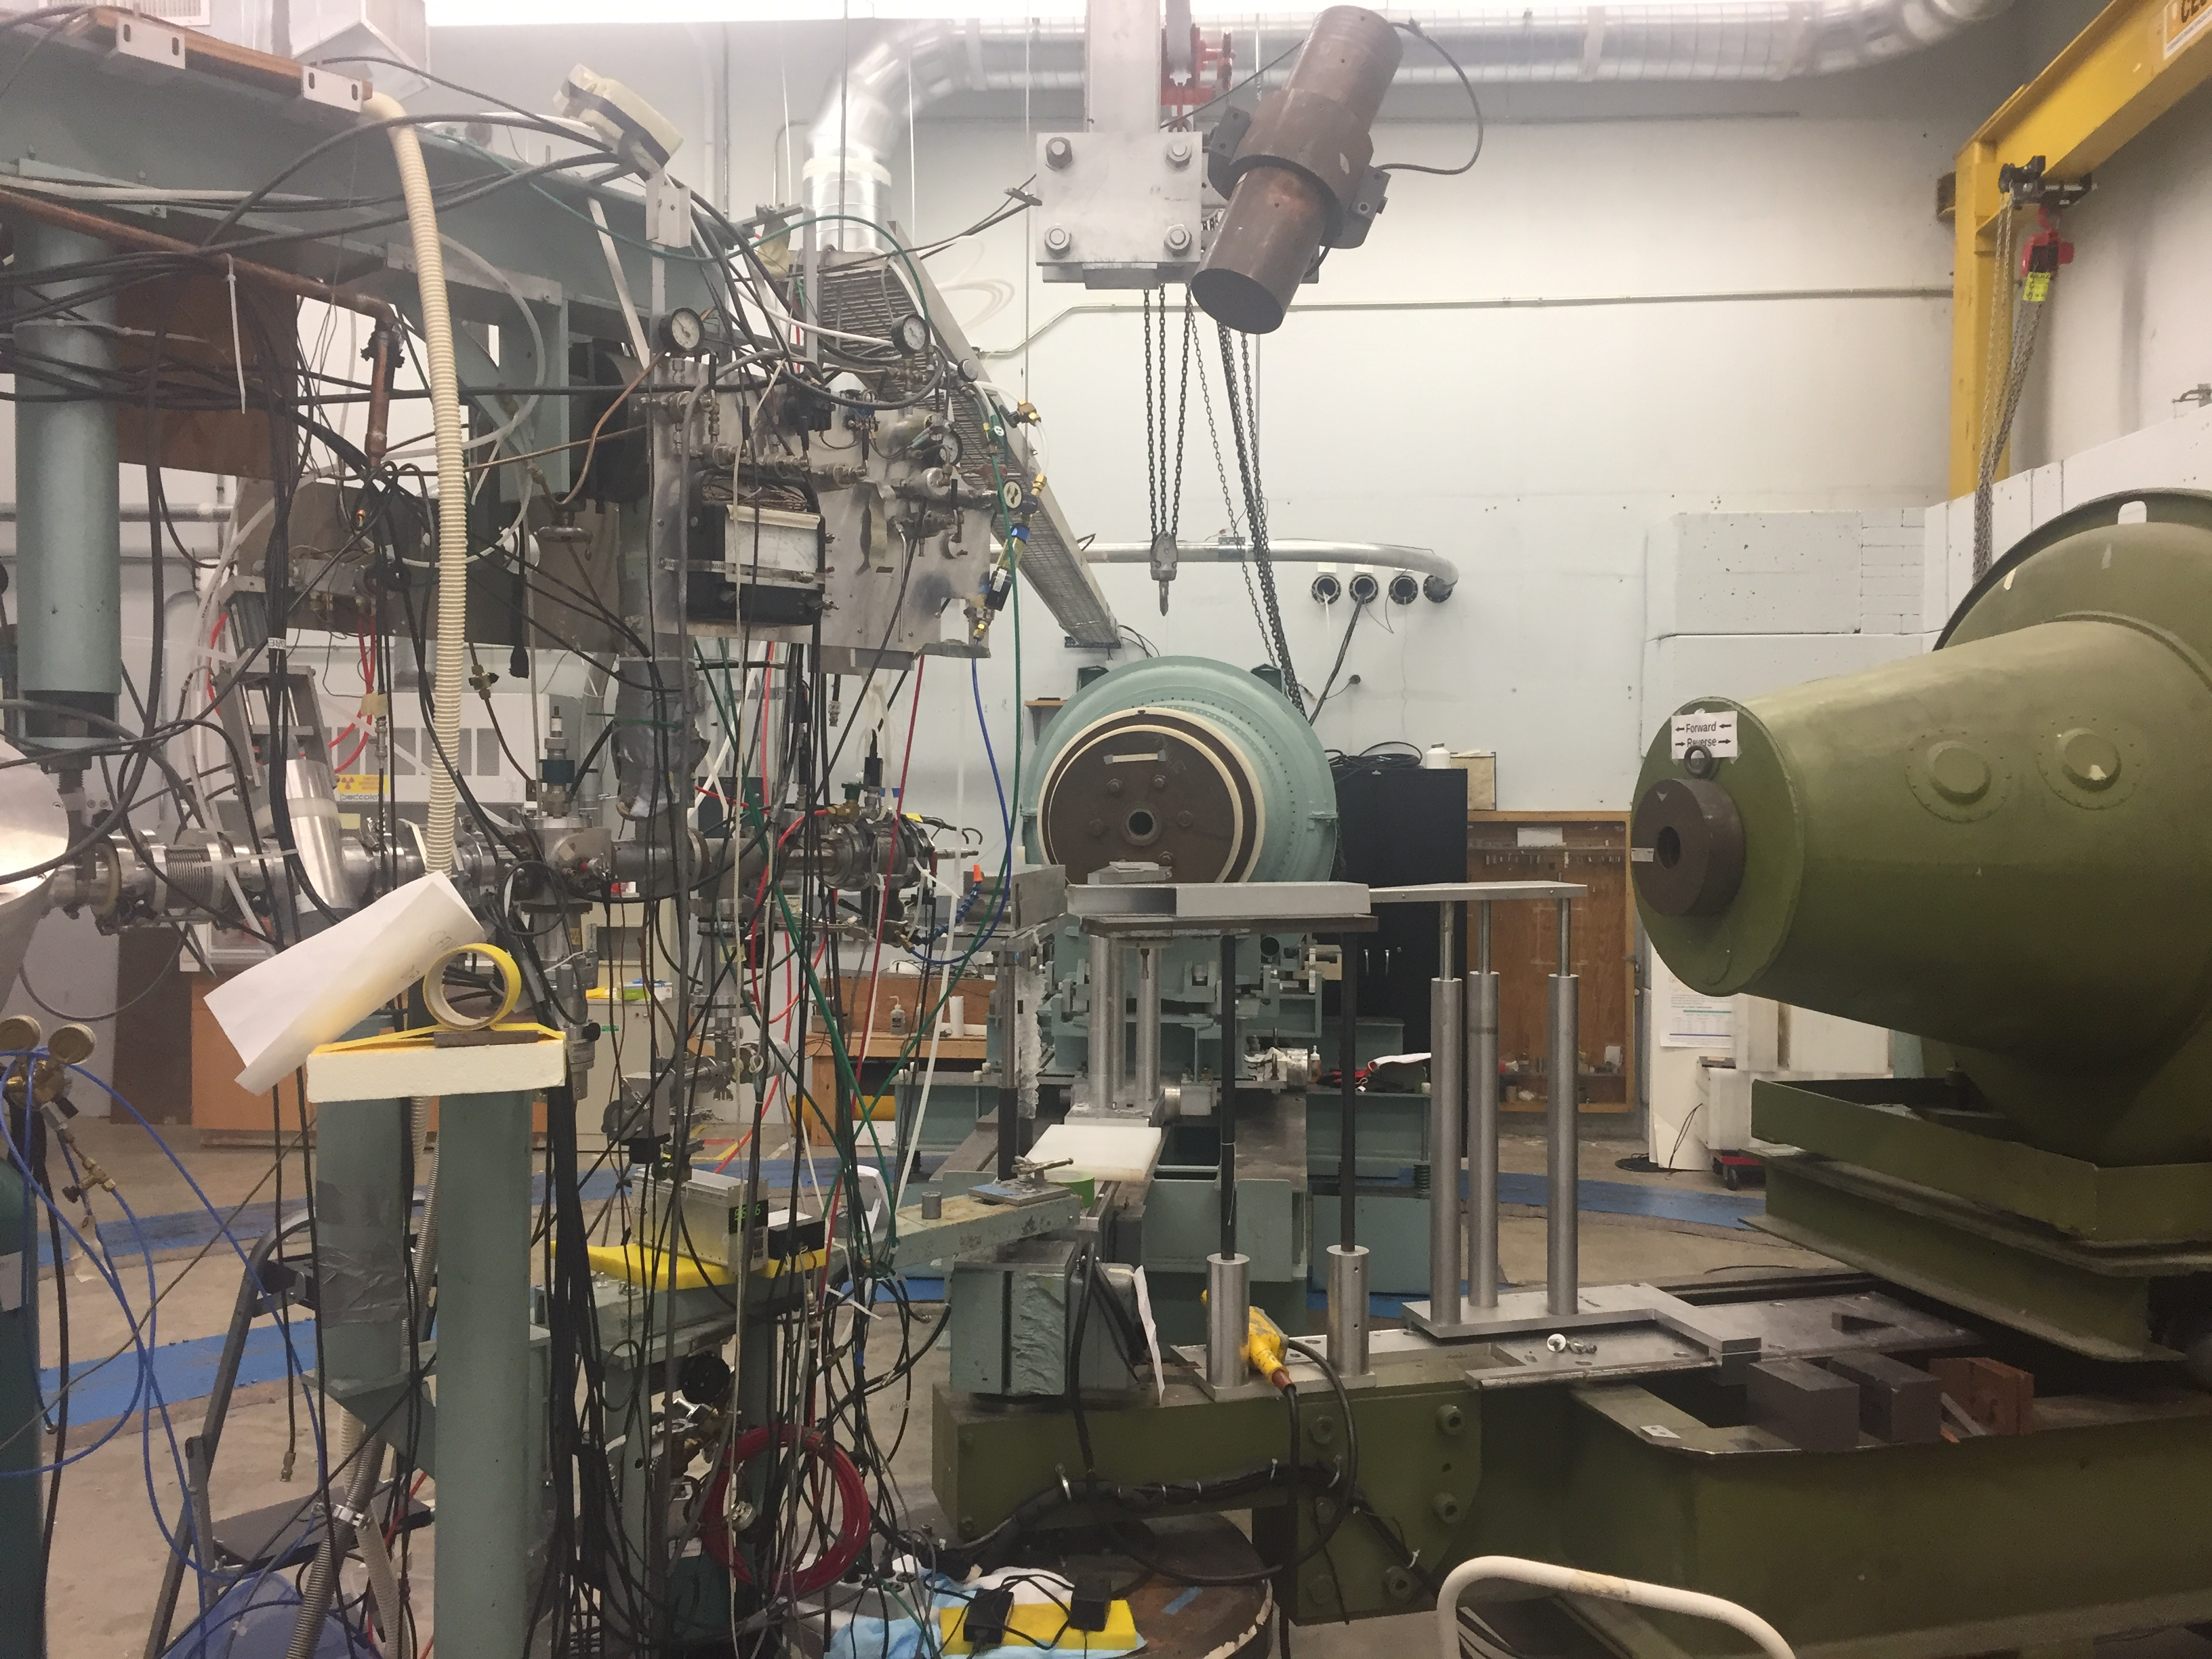
\includegraphics[width = 0.9\textwidth]{figures/TOFRoomPhoto.jpg}
    \caption[Image of the neutron TOF room at TUNL] 
    {
    Image of the neutron TOF room at TUNL. The deuteron beam pipe is visible on the left and
    terminates in a small deuteron gas target in the middle of the image, where neutrons are
    produced. The two detector arms are shown at center (6M) and right (4M). The ceiling
    monitor detector (CMON), which records beam flux, is visible at the top of the image.
    }
    \label{TOFRoomPhoto}
\end{figure}

\section{Data Acquisition}
Timing, pulse-shape discrimination, and pulse height information were
extracted by the analog signal processing logic laid out in \ref{ECSLogicDiagram}.
Raw signals from each neutron detector are processed by Mesytec MPD-4
pulse shape discrimination modules. The pulse tail length is converted to an
amplitude via a time-to-analog converter (TAC), providing neutron-gamma
discrimination. The pulse amplitude is measured by a separate
analog-to-digital converter (ADC). Event times (labeled "Gate" from each MPD-4)
are passed as logic signals to a single time-to-digital converter (TDC) so that
event times are recorded using a single clock. Pulse counts ("scalers") are
collected at each step and the TDC, ADC, and data acquisition computer busy
signals are used to arrest the TDC when the system is already busy processing,
avoiding event pile-up.

\begin{sidewaysfigure}[h]
    \centering
    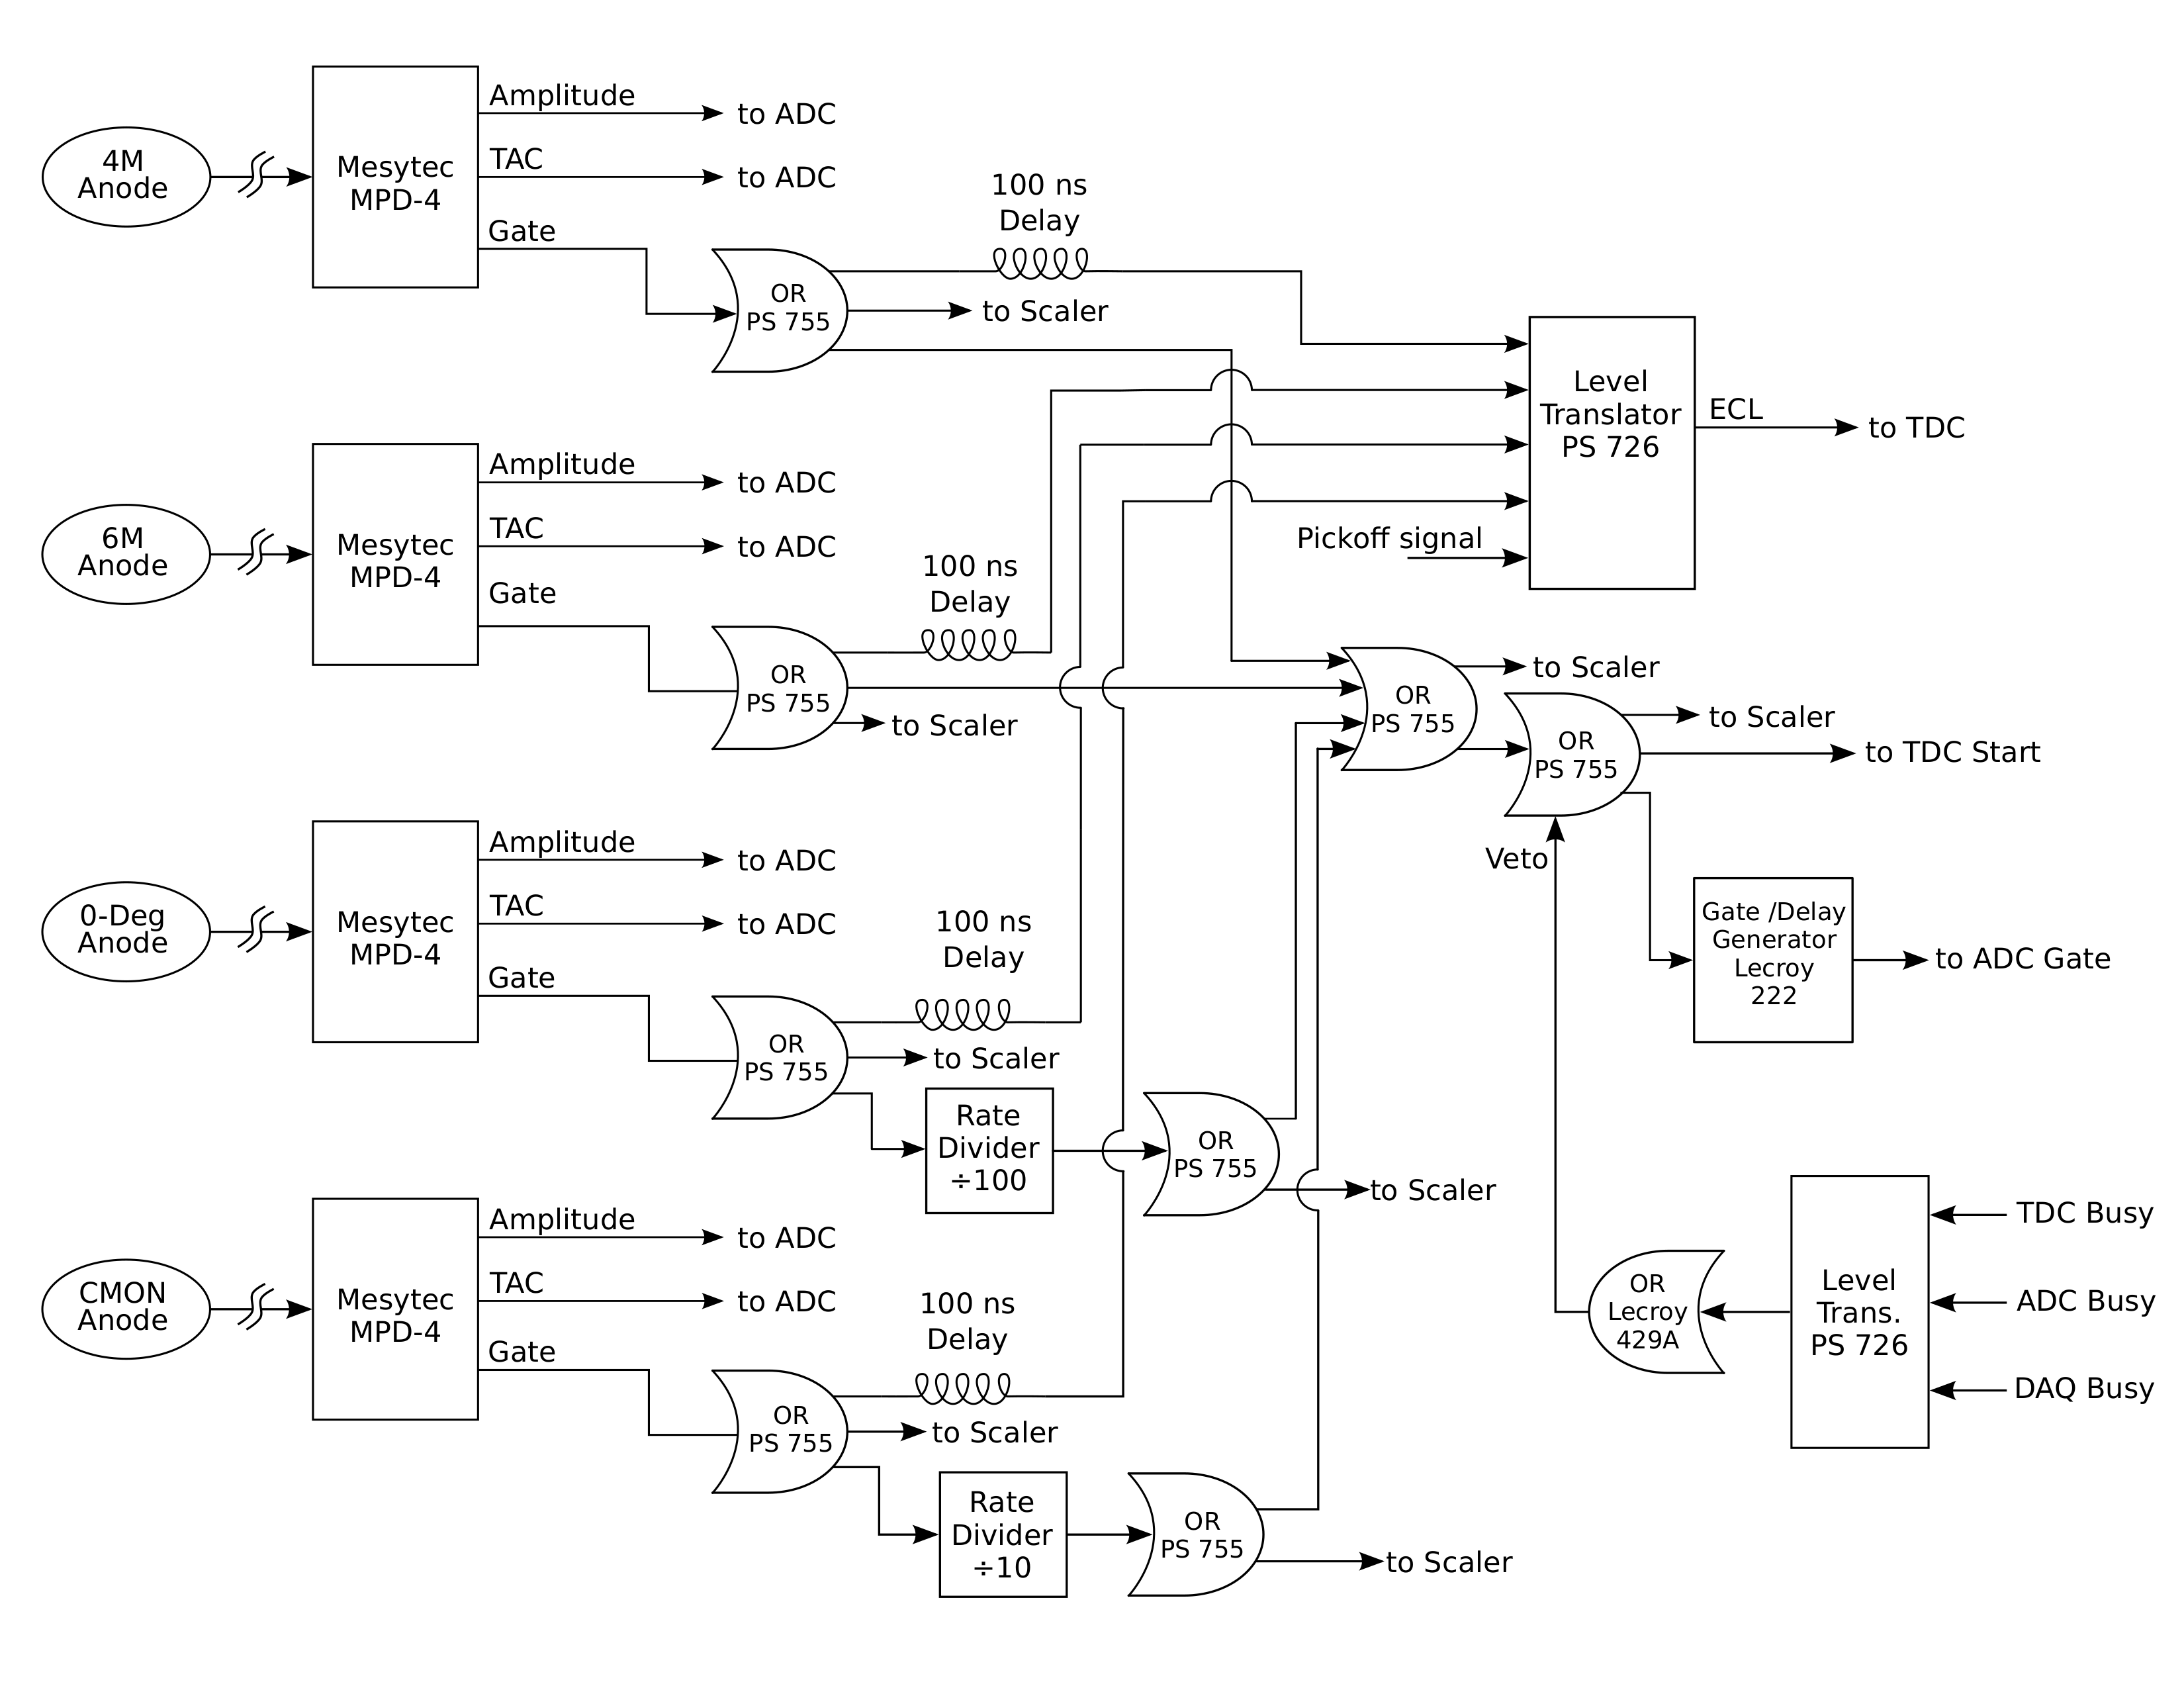
\includegraphics[width=0.9\textwidth]{figures/ECSLogic.png}
    \caption[Logic diagram for neutron \el\ data acquisition]
    {Logic diagram for neutron \el\ data acquisition at the TUNL time-of-flight
    room. Details are given in the text. Figure courtesy Ron Malone at TUNL.}
    \label{ECSLogicDiagram}
\end{sidewaysfigure}
